\subsection{Spatial Coupling Enables Candidate Compression}
\label{sec:eval-spatial}

This section validates the necessity of two key design choices in spatial coupling---window support ($W>1$) and contiguous structure---for candidate compression.

\paragraph{Choice of window width}
Spatial coupling through overlapping windows ($W \ge 2$) improves ranking
quality over per-section independent scoring ($W{=}1$), but the benefit
saturates and eventually reverses as $W$ grows. The underlying trade-off
is that a wider window reduces the number of top-ranked slots needed to
cover all dirty segments, yet simultaneously expands each slot's halo
neighborhood by a factor of $2W{-}1$; a net benefit requires the ranking
compression to outpace this geometric penalty. In our ablation, $W{=}2$
matches or improves upon $W{=}1$ in all tested configurations, with
larger gains under higher collision pressure---up to $\sim$3.8$\times$
candidate cost reduction. Beyond $W{=}2$, the compression headroom is
exhausted and halo expansion dominates when $L/B$ is tight (full ablation
in Supplement~\ref{sec:appendix-w-ablation}).


\paragraph{Contiguous vs.\ random grouping}
To isolate the contribution of contiguity, we compare two
mapping topologies at $W{=}4$: \emph{contiguous windows},
where each segment maps to $W$ adjacent sections starting
from a single hashed position, and \emph{random grouping},
where the $W$ sections are chosen independently and need not
be adjacent. The two share identical physical budget and
coverage; they differ only in spatial arrangement.
Complementary evidence from the energy-coverage view is
reported in Supplement Figure~\ref{fig:c1-5}.
The diff-capture curves in Figure~\ref{fig:c1-4} show that
contiguous windows yield a markedly steeper curve: 
contiguous mapping concentrates the energy of dirty segments
into localized peaks that are amplified by sliding-window
aggregation, whereas random grouping disperses that energy
and reduces separability under collision noise.
This aligns with the
matched-filter intuition from \S\ref{sec:spatial-coupling}:
random grouping breaks the coherent alignment of the
contiguous support, eliminating the superposition gain of
window aggregation.

\begin{figure}[!htbp]
\centering
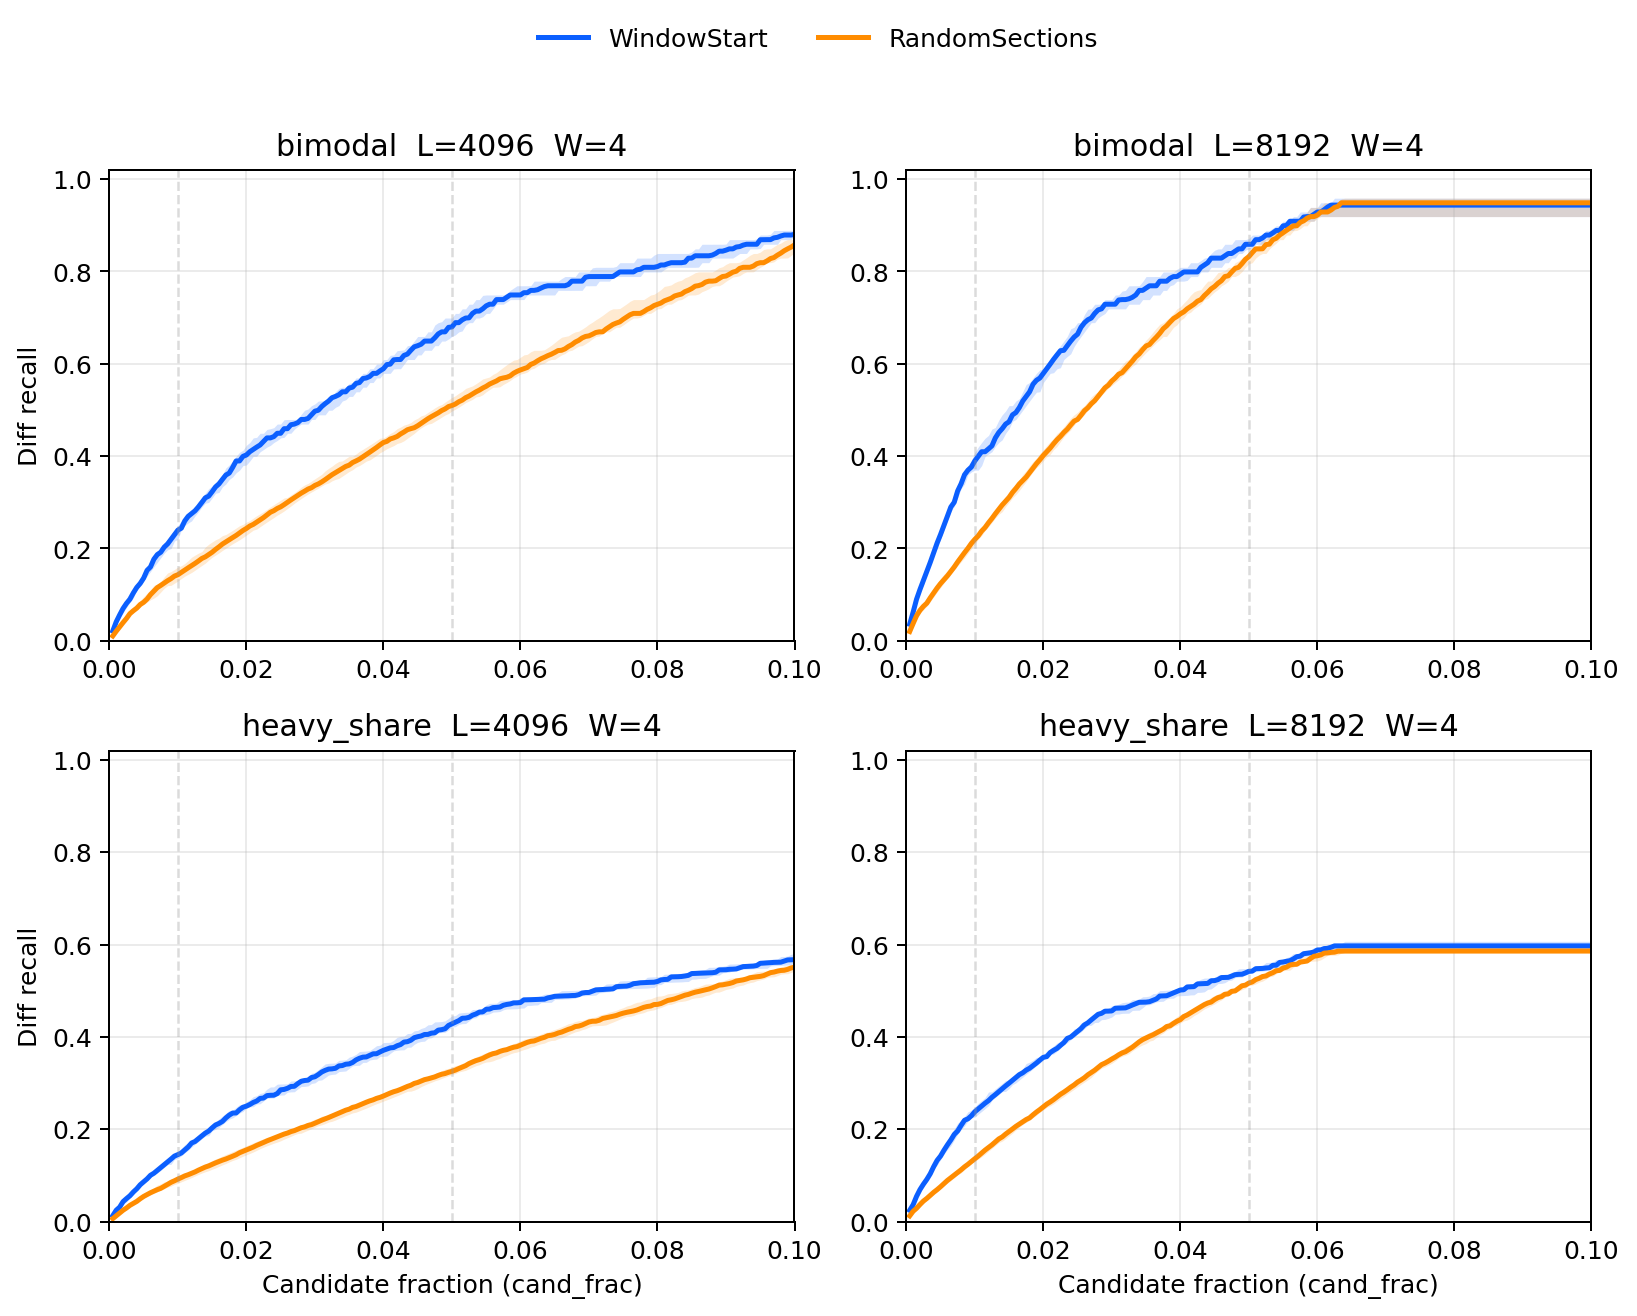
\includegraphics[width=0.95\linewidth]{figures/fig_topk_projected_window_coverage.png}
\caption{Diff capture curve: contiguous windows (\texttt{WindowStart}) vs.\ random grouping (\texttt{RandomSections}), $W{=}4$. 
Vertical axis: cumulative captured diff fraction. \texttt{bimodal} denotes concentrated pattern; \texttt{heavy\_share} denotes mixed pattern.}
\label{fig:c1-4}
\end{figure}

The trends from both experiments are consistent with the
scaling analysis in \S\ref{sec:spatial-coupling},
Equations~\eqref{eq:cand-expectation}--\eqref{eq:halo-prob},
although that analysis assumes sufficient signal separability.
When mixed or heavy-tail noise compresses the ranking margin,
the truncation quota needed to preserve recall increases, and
candidate cost rises accordingly; we characterize this
interaction further in \S\ref{sec:eval-operating}. Overall,
these results show that effective candidate compression depends
on both multi-section support ($W>1$) and contiguity, with the
main gain coming from coherent aggregation rather than simply
from increasing the number of sections touched by each segment.
